%
% This is the LaTeX template file for lecture notes for EE 382C/EE 361C.
%
% To familiarize yourself with this template, the body contains
% some examples of its use.  Look them over.  Then you can
% run LaTeX on this file.  After you have LaTeXed this file then
% you can look over the result either by printing it out with
% dvips or using xdvi.
%
% This template is based on the template for Prof. Sinclair's CS 270.

\documentclass[twoside]{article}
\usepackage{graphics}
\usepackage{graphicx}
\usepackage{hyperref}
\usepackage{listings}
\setlength{\oddsidemargin}{0.25 in}
\setlength{\evensidemargin}{-0.25 in}
\setlength{\topmargin}{-0.6 in}
\setlength{\textwidth}{6.5 in}
\setlength{\textheight}{8.5 in}
\setlength{\headsep}{0.75 in}
\setlength{\parindent}{0 in}
\setlength{\parskip}{0.1 in}

%
% The following commands set up the lecnum (lecture number)
% counter and make various numbering schemes work relative
% to the lecture number.
%
\newcounter{lecnum}
\renewcommand{\thepage}{\thelecnum-\arabic{page}}
\renewcommand{\thesection}{\thelecnum.\arabic{section}}
\renewcommand{\theequation}{\thelecnum.\arabic{equation}}
\renewcommand{\thefigure}{\thelecnum.\arabic{figure}}
\renewcommand{\thetable}{\thelecnum.\arabic{table}}

%
% The following macro is used to generate the header.
%
\newcommand{\lecture}[4]{
   \pagestyle{myheadings}
   \thispagestyle{plain}
   \newpage
   \setcounter{lecnum}{#1}
   \setcounter{page}{1}
   \noindent
   \begin{center}
   \framebox{
      \vbox{\vspace{2mm}
    \hbox to 6.28in { {\bf EE 382C/361C: Multicore Computing
                        \hfill Fall 2016} }
       \vspace{4mm}
       \hbox to 6.28in { {\Large \hfill Lecture #1: #2  \hfill} }
       \vspace{2mm}
       \hbox to 6.28in { {\it Lecturer: #3 \hfill Scribe: #4} }
      \vspace{2mm}}
   }
   \end{center}
   \markboth{Lecture #1: #2}{Lecture #1: #2}
   %{\bf Disclaimer}: {\it These notes have not been subjected to the
   %usual scrutiny reserved for formal publications.  They may be distributed
   %outside this class only with the permission of the Instructor.}
   \vspace*{4mm}
}

%
% Convention for citations is authors' initials followed by the year.
% For example, to cite a paper by Leighton and Maggs you would type
% \cite{LM89}, and to cite a paper by Strassen you would type \cite{S69}.
% (To avoid bibliography problems, for now we redefine the \cite command.)
% Also commands that create a suitable format for the reference list.
\renewcommand{\cite}[1]{[#1]}
\def\beginrefs{\begin{list}%
        {[\arabic{equation}]}{\usecounter{equation}
         \setlength{\leftmargin}{2.0truecm}\setlength{\labelsep}{0.4truecm}%
         \setlength{\labelwidth}{1.6truecm}}}
\def\endrefs{\end{list}}
\def\bibentry#1{\item[\hbox{[#1]}]}

%Use this command for a figure; it puts a figure in wherever you want it.
%usage: \fig{NUMBER}{SPACE-IN-INCHES}{CAPTION}
\newcommand{\fig}[3]{
			\vspace{#2}
			\begin{center}
			Figure \thelecnum.#1:~#3
			\end{center}
	}
% Use these for theorems, lemmas, proofs, etc.
\newtheorem{theorem}{Theorem}[lecnum]
\newtheorem{lemma}[theorem]{Lemma}
\newtheorem{proposition}[theorem]{Proposition}
\newtheorem{claim}[theorem]{Claim}
\newtheorem{corollary}[theorem]{Corollary}
\newtheorem{definition}[theorem]{Definition}
\newenvironment{proof}{{\bf Proof:}}{\hfill\rule{2mm}{2mm}}

% **** IF YOU WANT TO DEFINE ADDITIONAL MACROS FOR YOURSELF, PUT THEM HERE:

\begin{document}
%FILL IN THE RIGHT INFO.
%\lecture{**LECTURE-NUMBER**}{**DATE**}{**LECTURER**}{**SCRIBE**}
\lecture{13}{October 13}{Vijay Garg}{Nishanth Shanmugham}
%\footnotetext{These notes are partially based on those of Nigel Mansell.}

% **** YOUR NOTES GO HERE:

\section{Topics}

The topics covered in this lecture are:
\begin{itemize}
    \item GPUs and CUDA Introduction
    \item CUDA Hello World
    \item Parallel Computations in CUDA
    \item Terminology
    \item CUDA Threads \& Identification
    \item GitHub Links
\end{itemize}

\section{GPUs and CUDA Introduction}

Heteregenous computing is programming using both a CPU and a GPU. The
following terminology is commonly used to describe the CPU and GPU.

\begin{itemize}
    \item {\bf Host}: The CPU and its memory (host memory)
    \item {\bf Device}: The GPU and its memory (device memory)
\end{itemize}

\begin{figure}
  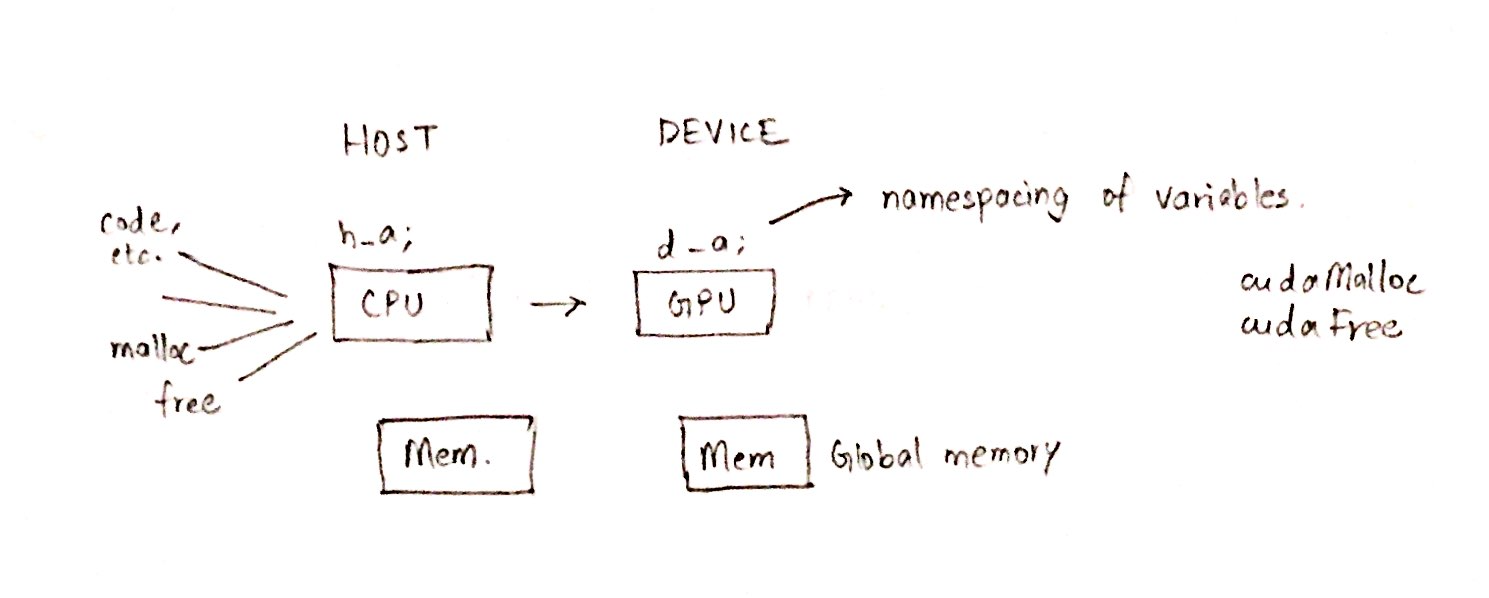
\includegraphics[width=\linewidth]{img/host_device.png}
  \caption{Host and Device}
\end{figure}

The general programming process is:

\begin{enumerate}
    \item Copy input data from CPU memory to GPU memory
    \item Load GPU program and execute,caching data on chip for performance
    \item Copy results from GPU memory to CPU memory
\end{enumerate}

The contents of this lecture can be found in {\tt
Introduction\_to\_CUDA\_C.pptx} on Canvas [Canvas]. This document aims to capture the
essential information from class---not to repeat the contents in the slides.

\section{Cuda Hello World}

\begin{verbatim}
__global__ void mykernel(void) {
}

int main(void) {
    mykernel<<1,1>>();
    printf(``hello, world\n'');
    return 0;
}
\end{verbatim}

The above code is a simple {\it Hello World} in CUDA in C. First, we declare
a function called {\tt mykernel}. The function is then invoked in {\tt
main}. 

\begin{center}
    {{\tt mykernel<<N,M>>(); }}
\end{center}


The first argument (N) in the angular brackets is the number of {\it
blocks} and the second argument (M) is the number of {\it threads per block}.

The {\tt \_\_global\_\_ } indicates that the function should be run of the
device; that is, {\tt mykernel} will be executed on the GPU. In this example,
the function does nothing. In future section, we write more useful programs.

\section{Parallel Computations in CUDA}

To run a CUDA function in parallel, we set the argument N (described above) to
a value greater than 1. This runs the function in parallel on N blocks on
the GPU. Making such a CUDA call can be considered the
equivalent of OpenMP's {\tt parallel for loop} construct.

\subsection{Addition}

The follwing code performs parallel addition on the GPU.

\begin{verbatim}
__global__ void add(int *a, int *b, int *c) {
    *c = *a + *b;
}


int main(void) {
	    int a, b, c;	            // host copies of a, b, c
	    int *d_a, *d_b, *d_c;	    // device copies of a, b, c
	    int size = sizeof(int);
	
	    // Allocate space for device copies of a, b, c
	    cudaMalloc((void **)&d_a, size);
	    cudaMalloc((void **)&d_b, size);
	    cudaMalloc((void **)&d_c, size);

	    // Setup input values
	    a = 2;
	    b = 7;

	    cudaMemcpy(d_a, &a, size, cudaMemcpyHostToDevice);
	    cudaMemcpy(d_b, &b, size, cudaMemcpyHostToDevice);

	    // Launch add() kernel on GPU
	    add<<<1,1>>>(d_a, d_b, d_c);

	    // Copy result back to host
	    cudaMemcpy(&c, d_c, size, cudaMemcpyDeviceToHost);

	    // Cleanup
	    cudaFree(d_a); cudaFree(d_b); cudaFree(d_c);
	    return 0;
}
\end{verbatim}

Since the {\add} function runs on the device the variables used in the
function should reside in device memory. Hence we use the {\tt cudaMalloc}
and {\tt cudaFree} functions to allocate and release memory on the device.
Moreover, after allocating the memory, the values should be copied from the
host to the device using {\tt cudaMemcpy}. Similarly, after the computation
is complete and before releasing the device memory, the result must be
copied to the host using {\tt cudaMemcpy}. The direction that {\tt cudaMemcpy}
should use is specified using the last argument; in this case {\tt
cudaMemcpyHostToDevice} and {\tt cudaMemcpyDeviceToHost}.

\section{Terminology}

When a GPU is started, a {\tt grid} is started. Figure 13.2 displays the
logical construction in a GPU. A grid is made of a set of {\tt blocks}. A
block consists of a set of {\tt threads}.

\begin{figure}
  
\includegraphics[width=\linewidth]{img/lc.png}
  \caption{Logical construction}
\end{figure}

\subsection{Hardware}

As show in Figure 13.1, the blocks of a grid are enumerated and distributed to 
multiprocessors. Shared memory s local to a block. Accessing shared memory
is faster than going to global memory. A streaming multiprocessor is composed of
multiple streaming processes.

\begin{figure}
  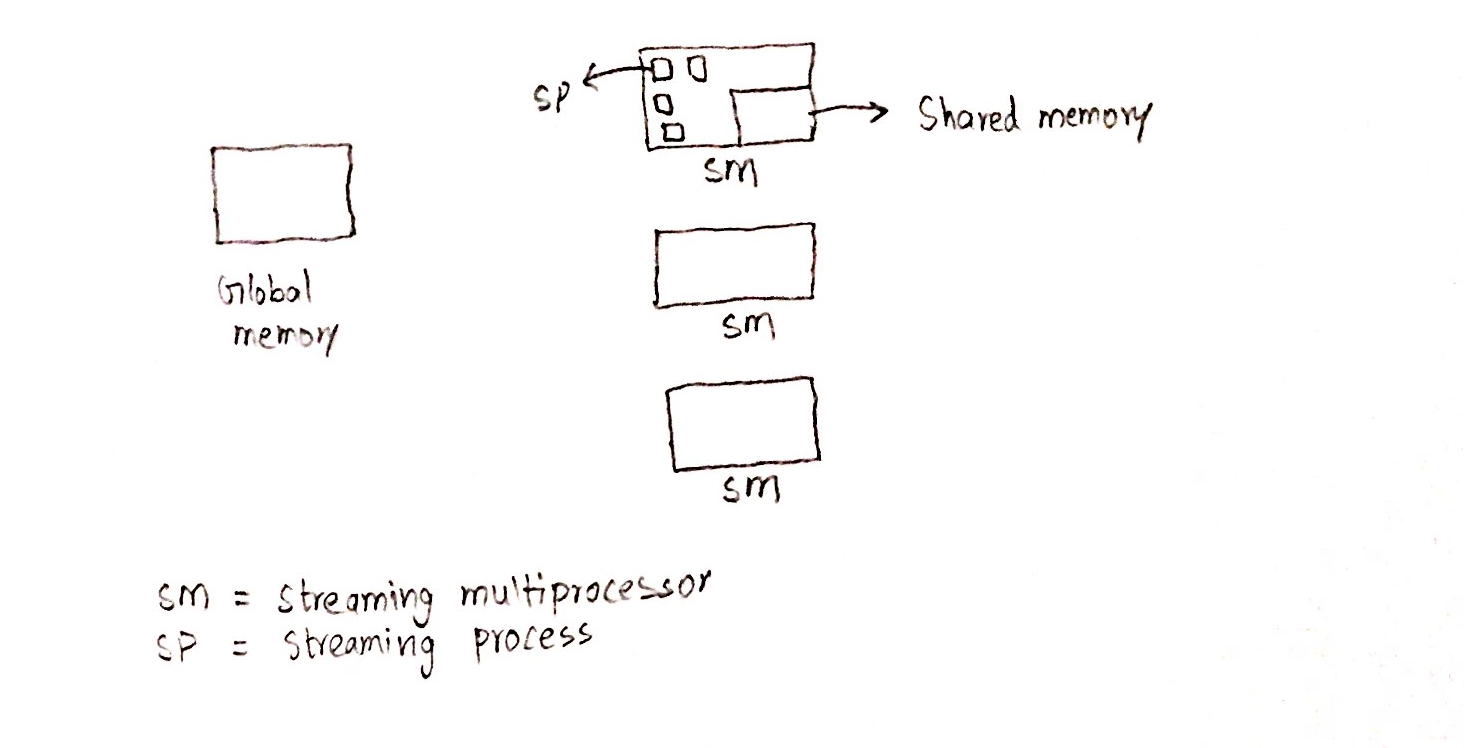
\includegraphics[width=\linewidth]{img/hardware.png}
  \caption{Hardware}
\end{figure}

\section{CUDA Threads \& Identification}

A block can be split into parallel threads. However, there is a restriction
on the maximum number of threads that can run in a single block. If such a
situation arises, an option is to use multiple blocks.

Unlike blocks, threads can communicate and sychronize.

In addition, the following tips are useful:

\begin{enumerate}
    \item If the work is dependent between parallel workers, use the same
        block. This provides the advantage of shared memory access
        and communication between threads in the block.
    \item If the work is not dependent, then using multiple blocks is
        faster.
\end{enumerate}

\subsection{Identifying blocks and threads}

The predefined variables {\tt blockIdx}, {\tt blockDim}, and {\tt
threadIdx} can be used to designate IDs to threads running in parallel. This
allows programmers to assign tasks to each thread based on their ID.

For instance, the index that a paritcular thread should work on can be
computed using:

\begin{center}
    {{\tt int index = threadIdx.x + (blockIdx.x * blockDim.x); }}
\end{center}

In addition to the {\tt .x} field, {\tt .y} and {\tt z} fields are also
available to facilitate working with multi-dimensional data.

\subsection{More Terms}

\begin{itemize}
    \item {\bf \_\_shared\_\_}: Declares a variable/array as shared memory..
        \begin{itemize}
            \item Data is shared between threads in a block.
            \item Data is not visible to threads in other blocks.
        \end{itemize}
    \item {\bf \_\_syncthreads()}: Used as a barrier to wait for threads to prevent data
        hazards. Similar to the Java construct Threads#join.
\end{itemize}

\section{GitHub links and Conclusion}

The files on GitHub have Cuda examples [GitHub]. See the directory named
{\tt cuda}. The code documented with comments. For additional explanation of
{\tt reduce.cu}, see the next lecture.

\section*{References}
\beginrefs
\bibentry{GitHub}{} Multicore Computing source code, {\it https://github.com/vijaygarg1/UT-Garg-EE382C-EE361C-Multicore}
\bibentry{Canvas}{} Introduction to CUDA, {\it https://utexas.instructure.com/courses/1174768/modules/items/8255450}
\bibentry{Cuda}{} Cuda Toolkit Documentation{\it
http://docs.nvidia.com/cuda/index.html#axzz4NfgY7FeW}
\endrefs


\end{document}
